% MIS pdf comparison figure
\begin{figure*}[t]
	\addtolength{\tabcolsep}{-4pt}
	\begin{tabular}{ccc}
		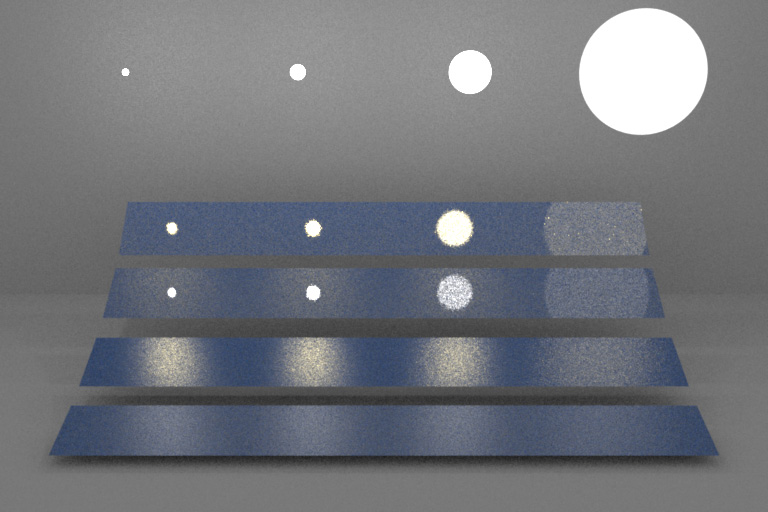
\includegraphics[width=0.32\textwidth]{img/validations/mis/mi_acr_64spp_14min.jpg} & 
		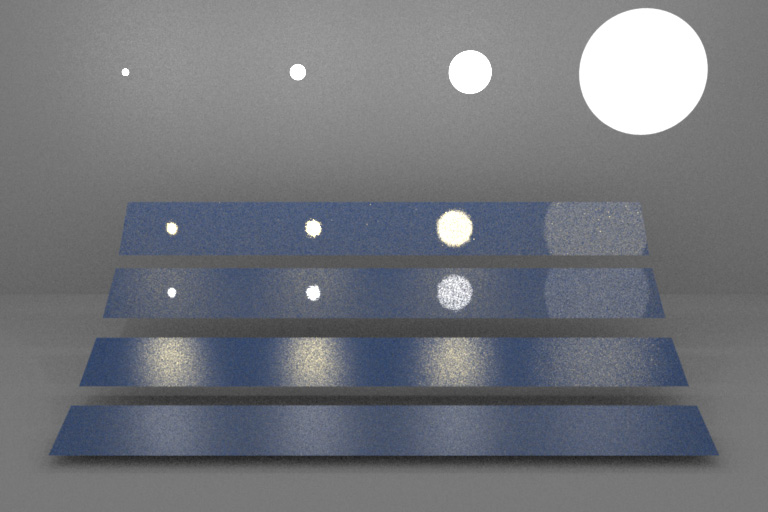
\includegraphics[width=0.32\textwidth]{img/validations/mis/mi_trt_64spp_4_1min.jpg} & 
		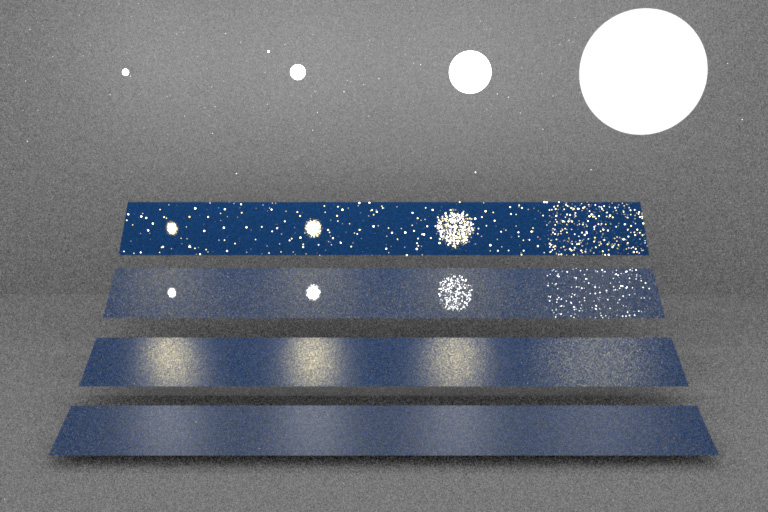
\includegraphics[width=0.32\textwidth]{img/validations/mis/mi_noMIS_80spp_4_2min.jpg} \\
		MIS + unbiased pdf (14 min) &
		MIS + approx. pdf (4 min) &
		no MIS (4 min) \\ 
	\end{tabular}
	\caption{
		\textbf{Multiple importance sampling} using our BSDFs.
		\sz{The slabs in this figure use a layered material with rough dielectric on the top, rough gold conductor on the bottom, and blueish homogeneous scattering medium in between.}
		\textbf{Left:} Using the unbiased pdf from \S\ref{sssec:ours_pdf_unbiased} for MIS in a traditional global path tracer. \textbf{Middle:} Using the approximate pdf from \S\ref{sssec:ours_pdf_approx} is faster and gives equivalent quality. \textbf{Right:} Using no MIS is clearly inferior.}
	\label{fig:pdf-eval}
\end{figure*}